 \documentclass[12pt,a4paper]{article}

\usepackage{setspace}
\onehalfspacing
\usepackage{caption}
\usepackage{subcaption}
\usepackage{float}
\captionsetup[table]{font={stretch=1.5}}     %% change 1.5 as you like
\captionsetup[figure]{font=onehalfspacing}    %% change onehalfspacing as you like
\usepackage[english]{babel}
\usepackage[utf8]{inputenc}
\usepackage{amsmath}
\usepackage{mathtools}
\usepackage{amssymb}
\usepackage{graphicx}
\usepackage{braket}
\usepackage[colorinlistoftodos]{todonotes}
\usepackage[top=1.0in,left=1.0in,right=1.0in,bottom=1.0in]{geometry}
\usepackage[
backend=biber,
style=numeric,
citestyle=ieee,
subentry,
mcite=true,
]{biblatex} %biblatex, more modern form of bibtex 
\usepackage{multicol,caption}
\usepackage{makeidx}
\usepackage{pdfpages}
\usepackage[compat=1.0.0]{tikz-feynman}
\usepackage{hyperref}
%\usepackage{LuaLaTeX}
\makeindex
%\usepackage{fixltx2e}
%\usepackage{cite} %if you want to use bibtex
\newenvironment{Figure}
  {\par\medskip\noindent\minipage{\linewidth}}
  {\endminipage\par\medskip}
\setlength{\columnsep}{1cm}
\setlength{\parindent}{0pt}
\usepackage{color,soul}
\usepackage{booktabs}
\newcommand{\ra}[1]{\renewcommand{\arraystretch}{#1}}
% \defbibentryset{griffiths2008book}{griffiths2008introduction, griffiths2008neutrino1.5, griffiths2008neutrinoOscillations} %if you want to use biblatex with multiple referances, useful for books
\addbibresource{refs.bib} %if you want to use bib latex, add sources
\setlength\bibitemsep{2.0\itemsep} % if you want to use bib latex and increase item seperation

\title{Re-purposing an Anti-Neutrino Detector for Cosmic Muon Tomography to Discern Specific Reactor Buildings and Features}
\date{\today}
\author{Ronald Collins and Yan-Jie Schnellbach, Carl Metelko, Jon Coleman, \\George Holt}

\begin{document}
\maketitle


\begin{center}
\textit{University of Liverpool, Department of Physics,\\}
\textit{VIDARR collaboration\\}
\end{center}
 

% \pagenumbering{gobble}
% \newpage
% \pagenumbering{roman}
\begin{abstract}
\normalsize During the deployment at Wylfa between 2014 -- 2016 a prototype anti-neutrino detector (a prototype of VIDARR) took cosmic muon data in accidental coincidence with the anti-neutrino measurements. From 2016 -- 2018 the same detector took data at the University of Liverpool. By taking the ratio of these two data sets and using Geant4 simulations it is possible to discern specific buildings, building heights, and features at the Wylfa reactor site including the reactor core/reactor core apparatus.\\

\providecommand{\keywords}[1]{\textbf{\textit{Keywords:}} #1} %Keywords command has to be supplied manually
\keywords{Monte Carlo, Geant4, cosmic muon tomography}
\end{abstract}
\vspace{5mm} %5mm vertical space before main body of text

% \newpage

\pagenumbering{arabic}

\section{A Brief Overview of the Detector}
The 1 tonne scale anti-neutrino detector deployed at the Wylfa reactor site was $\sim$ 60\,m from the 1.5\,GW$_{th}$ reactor. It was a prototype of the VIDARR detector based on the ND280 electromagnetic calorimeter from T2K. Using segmented extruded plastic scintillator and Hamamatsu Multi-Pixel Photon Counters (MPPCs). The detector had 49 layers of plastic scintillator which alternated being at 90$^\circ$ from the previous layer. The active detector region has gadolinium sheets in-between the layers of plastic in order to capture neutrons and analyse the anti-neutrinos through inverse $\beta$ decay. Muons interact with the detector as minimally ionising particles (MIPs) as determined by the Bethe-Bloch formula. Muons were primarily as a calibration tool at the beginning of the deployment\cite{Carroll_2018}. During the main deployment at Wylfa cosmic muons (both $\mu^+$ and $\mu^-$ as the detector cannot distinguish between the two) are mostly excluded via a cosmic muon veto in order to reduce background when measuring anti-neutrinos. As a result the amount of information available is significantly less than the 20 month period of deployment at Wylfa would suggest. Instead the number of cosmic muon events is more proportional to $sim$ 3 hours worth of live time. 
 
\section{One Sided Cosmic $\mu$ Tomography}
Cosmic $\mu$ tomography has two distinct types one sided and two sided. Two sided tomography typically requires detectors with much larger area than the object attempting to be measured in order to calculate $\mu$ scattering and vertex reconstruction \cite{schultz_2007}. However the size of the reactor site buildings is far greater than the size of the VIDARR detector as a result one sided cosmic $\mu$ tomography will be used instead seen in figure \ref{fig:oneSidedMuTomography}. DIAPHANE has used one sided cosmic $\mu$ tomography to analyse volcanic mountains seen in figure \ref{fig:DIAPHANE_mountianImages}. The technique DIAPHANE used requires months/years of data via the use of $\mu$ radiography \cite{Marteau_2017}. 

\begin{figure}[H]
 \centering
 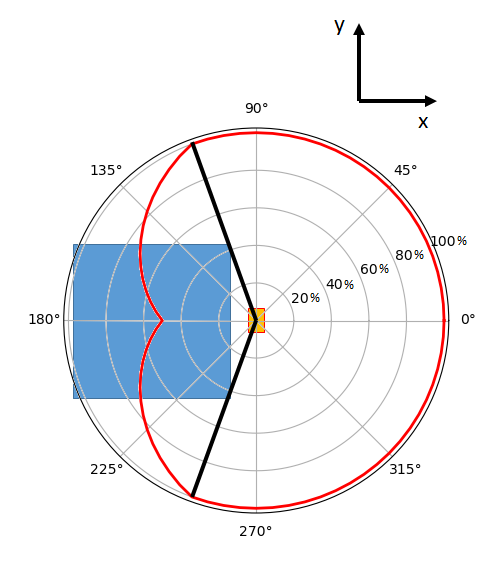
\includegraphics[width=0.5\linewidth]{oneSidedMuTomography.png}
 \captionof{figure}{A top down theoretical example of what one sided cosmic $\mu$ tomography looks like. The more material that cosmic $\mu$ have to pass through the lower chance they will be detected via attenuation.} 
 \label{fig:oneSidedMuTomography}
\end{figure}

\begin{figure}[H]
 \centering
 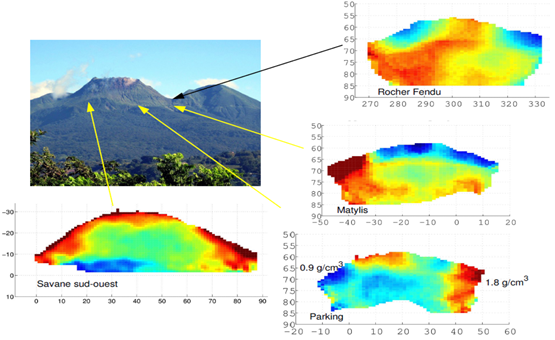
\includegraphics[width=1.0\linewidth]{DIAPHANE_mountainImages.png}
 \captionof{figure}{Results from DIAPHANE measuring the Soufrière of Guadeloupe from \cite{Marteau_2017}. } 
 \label{fig:DIAPHANE_mountianImages}
\end{figure}

\section{Wylfa Reactor Site} \label{sec:wylfaReactorSite}
During July of 2014 the VIDARR prototype detector started taking data at the Wylfa reactor site. A cut away of the Wylfa reactor building can be seen in figure \ref{fig:WylfaCutAway}. In figure \ref{fig:WylfaCutAway} the structure of the main reactor building is significantly denser in the bottom half of construction than the top half. The upper storage section therefore will block fewer cosmic $\mu$ than bottom section with the reactor. This structure impacts the outline of the shadow as the main reactor building does have less of an effect than some of the service buildings that are closer to the detector. This means that measuring the main reactor building height is more difficult than measuring the height of the service buildings closer to the detector. The position of the detector can be seen from google maps in figure \ref{fig:googleMapsDetector}. There are many buildings that will cast shadows on the detector. This combined with the low density of the upper storage section of the Wylfa reactor building means that the shadow analysis is more complex than might be expected. 

\begin{figure}[H]
 \centering
 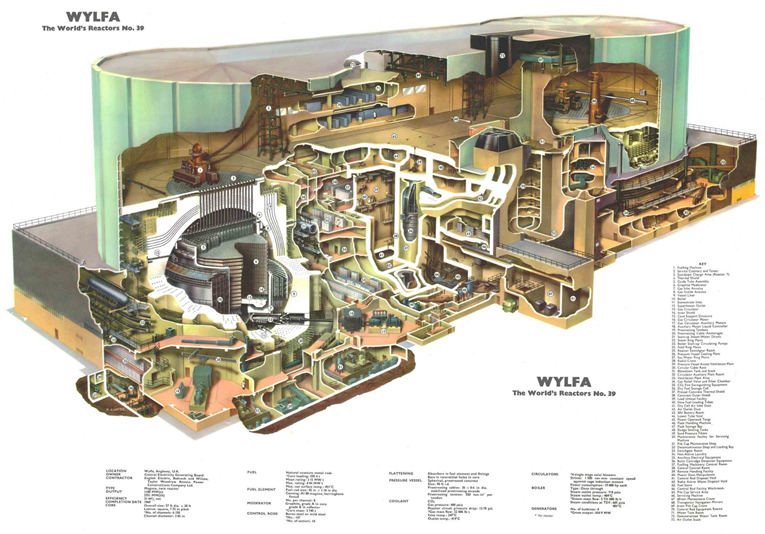
\includegraphics[width=1.0\linewidth]{wylfaReactorBuildings/wylfaReactorRoughStructure.png}
 \captionof{figure}{A cut away diagram from \cite{neiMag_1965}. Shows the internal structure of the Wylfa from the back of the reactor buildings the bottom half of the reactor buildings have thick concrete walls whilst the upper section is mostly storage. This cutaway is from a magazine. So it should only be taken as a rough approximation of the Wylfa reactor building.} 
 \label{fig:WylfaCutAway}
\end{figure}

\begin{figure}[H]
 \centering
 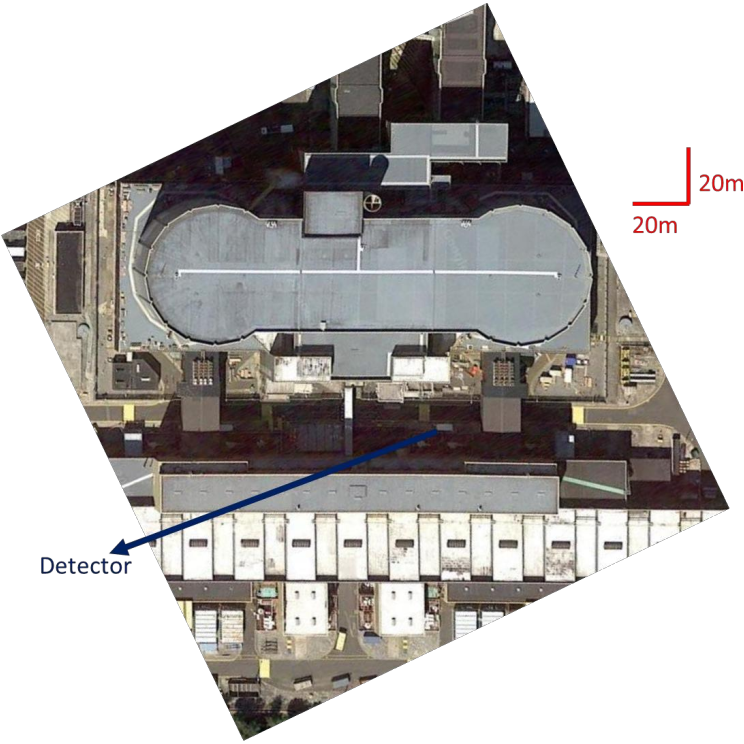
\includegraphics[width=0.7\linewidth]{wylfaReactorBuildings/wylfaTraceStep0.png}
 \captionof{figure}{Google image satellite picture taken from the web. The detector is in the middle of many site buildings that will cast shadows on it.} 
 \label{fig:googleMapsDetector}
\end{figure}

\section{Geant4 Geometry} \label{sec:geant4Geometry}
In order to combat the complexity of the reactor site Geant4 \cite{Agostinelli:2002hh} is used to simulate each building individually. The overall setup for the buildings in Geant4 can be seen in figures \ref{fig:WylfaSideOnG4} and \ref{fig:WylfaTopDownG4}. Approximations for the sizes in x and y in Geant4 are estimated from the google maps satellite image seen in figure \ref{fig:googleMapsDetector}. The heights of the buildings have to be approximated from the data measured at Wylfa, this is then compared and adjusted until the heights of the shadows roughly match the heights of the shadows at Wylfa. Heights represented in figures \ref{fig:WylfaSideOnG4} and \ref{fig:WylfaTopDownG4} are 25\,m for turbine hall, 45\,m for main reactor building, 45\,m for service towers, 50\,m for back service building, 35\,m for service buildings, 10\,m off the ground for steam bridges with them being 5\,m thick in the z axis. 

\begin{figure}[H]
 \centering
 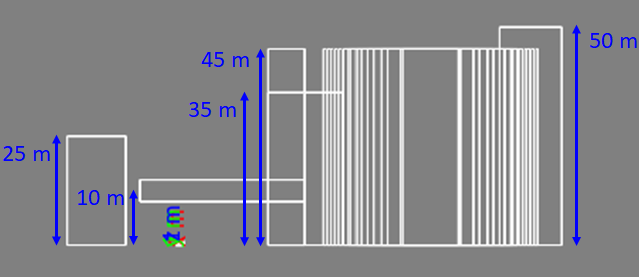
\includegraphics[width=0.6\linewidth]{wylfaReactorBuildings/WylfaG4GeometryHeight.png}
 \captionof{figure}{Geant4 x z side on view of the reactor buildings where the reactor buildings are 100\,\% concrete.} \label{fig:WylfaSideOnG4}
\end{figure}

\begin{figure}[H]
 \centering
 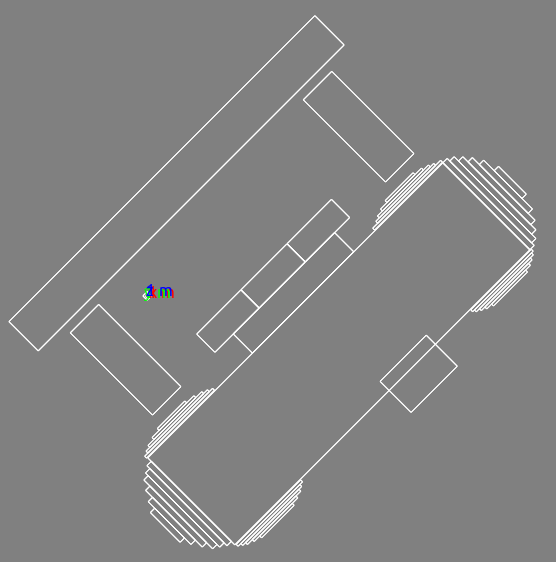
\includegraphics[width=0.5\linewidth]{wylfaReactorBuildings/WylfaTopDownGeomRedoCut.png}
 \captionof{figure}{Geant4 x y top down view of the reactor buildings where the reactor buildings are 100\,\% concrete.} \label{fig:WylfaTopDownG4}
\end{figure}

\section{Reconstruction of Cosmic $\mu$ Tracks} \label{sec:ReconstructionOfCosmicMuTracks}
The cosmic $\mu$ tracks are reconstructed with a custom built tracker. The tracker has two main purposes to run as a continuous online track fitter to allow for constant calibration of the detector (excluding showers) and to perform a full reconstruction of cosmic tracks (including showers). The basic logic chain for fitting each individual track is as follows: 
\begin{description}
  \item[1.] Exclude all hits below 0.345\,MeV
  \item[2.] Exclude hits that are 4 bars away from any other hit 
  \item[3.] Exclude events that have $<$ 4 bars per side that are above a 0.69\,MeV threshold
  \item[4.] Find a basic gradient and intercept using top and bottom hit of the event
  \item[5.] First basic fit of the track 
  \item[6.] Exclude hits that are 4.5 bars away from the track and do second fit 
  \item[7.] Exclude any hits that are 0.5 bars away from the track
  \item[8.] Third and final fit 
\end{description}

For the following analysis showering events were considered as well. This is due to the low statistics when taking cosmic $\mu$ in accidental coincidence. For calibration a $\chi^2$ cut would also be implemented. 

\section{Ratios of Measured and Simulated Data Sets} \label{sec:RatiosOfMeasuredAndSimulatedDataSets}
In order to highlight the shadows effectively taking the ratio of two data sets is required. Figure \ref{fig:pvtWylfaAndLiverpool} shows the distortion inherent to analysing the cosmic $\mu$ distribution with the detector both at Liverpool (\ref{subFig:pvtLiverpool}) and at Wylfa (\ref{subFig:pvtWylfa}). This distortion has 3 main components Firstly the cosmic $\mu$ distribution is a spherical distribution which is being analysed by a cubiod shaped detector. Secondly the VIDARR prototype segments were 4\,cm wide by 1\,cm tall by 152\,cm long as a result there is a limit to the angular resolution which causes bin migration. This bin migration is most clearly seen in bins $\phi$ = 0$^\circ$, $\phi$ =  90$^\circ$, $\phi$ = 180$^\circ$, $\phi$ = 270$^\circ$ in both figure \ref{subFig:pvtLiverpool} and figure \ref{subFig:pvtWylfa}. Thirdly there is significant scattering as the cosmic $\mu$ interact with the atmosphere and buildings which causes blurred edges. Therefore the shadows in the wylfa data set in figure \ref{subFig:pvtWylfa} are significantly fainter than would be expected for such large and dense buildings.  

\begin{figure}[H]
\centering
\begin{subfigure}{.5\textwidth}
  \centering
  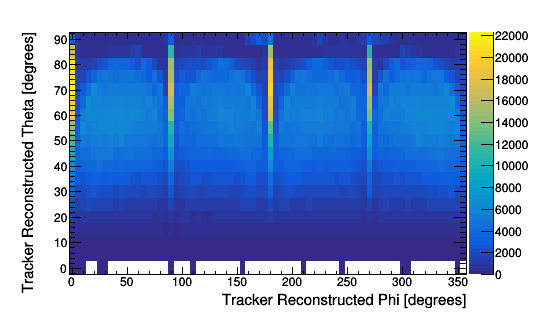
\includegraphics[width=\linewidth]{ReconstructedPhiTheta/pVsTLiverpoolRedo.png}
  \captionsetup{width=.9\linewidth}
  \caption{Liverpool cosmic $\mu$ data of reconstructed $\phi$ vs. $\theta$ by the cosmic tracker. Shadows are present in this data but are very faint and are below 20$^{\circ}$ $\theta$.}
  \label{subFig:pvtLiverpool}
\end{subfigure}%
\begin{subfigure}{.5\textwidth}
  \centering
  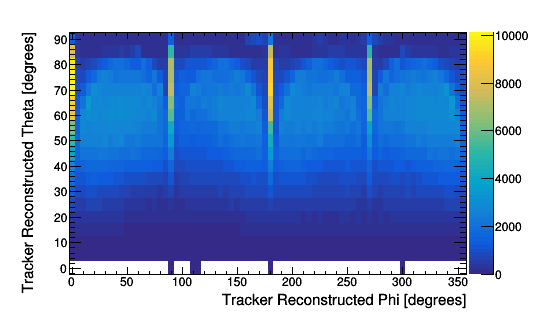
\includegraphics[width=\linewidth]{ReconstructedPhiTheta/pVsTWylfaRedo.png}
  \captionsetup{width=.9\linewidth}
  \caption{Wylfa cosmic $\mu$ data of reconstructed $\phi$ vs. $\theta$ by the cosmic tracker. Strong shadows are present in this data from 0$^{\circ}$ $\theta$ to 60 $^{\circ}$ $\theta$.}
  \label{subFig:pvtWylfa}
\end{subfigure}
\caption{The azimuthal angle ($\phi$) and the polar angle ($\theta$) for the Liverpool and Wylfa cosmic Muon distributions. Both distributions are warped considerably due to the shape and segmentation of the detector.}
\label{fig:pvtWylfaAndLiverpool}
\end{figure}

According to the CRY library \cite{ieee_cry_2007} 161867 $\mu^-$ and 174291 $\mu^+$ are produced in 2824.79\,s for 1 m\,$^2$ VIDARR's area is 1.52\,m $\times$ 1.52\,m = 2.3104\,m$^2$ resulting in $\sim$ 275 muons s$^{-1}$ the Wylfa data has $\sim$ 3 $\times$ 10$^6$ events and so is only $\sim$ 3 hours worth of live time. At the Wylfa reactor site there are several buildings and features that are expected to produce shadows which figure \ref{fig:wylfaTraceOfBuildings} shows with a corresponding key. By simulating each building in Geant4 it is possible to obtain an outline of each building shown in figure \ref{fig:wylfaTraceOfBuildings} as it would be visible to the detector. Then all the buildings can be simulated at once taking the ratio both with and without the buildings highlighting the outline in $\phi$ and $\theta$ as it appears to the detector which figure \ref{fig:simulatedBuildingsThetaPhi} shows. Finally the Wylfa data is then divided by the Liverpool data which is normalised to the number of events in the Wylfa data set this produces the results seen in figure \ref{fig:measuredBuildingsThetaPhi} each component is then visible for each individual building. The simulated 360$^\circ$ panoramic (figure \ref{fig:simulatedBuildingsThetaPhi}) and the measured 360$^\circ$ panoramic (figure \ref{fig:measuredBuildingsThetaPhi}) match each other very closely. Suggesting the shadows shown in figure \ref{fig:measuredBuildingsThetaPhi} are likely an accurate representation of the Wylfa reactor site.
\\\\The feature of most interest is the reactor core which is shown by the thin red line in figure \ref{fig:measuredBuildingsThetaPhi}. This feature is however significantly taller than would be expected it is therefore assumed that the reactor core apparatus is also adding to the shadow as well. The reactor core shielding can also be seen around the core at lower angles of $\theta$ = 20$^\circ$ and $\theta$ = 25$^\circ$ also highlighting the core's position effectively. With the other buildings accounted for in the shadow it is reasonable to assume that this feature is the reactor core. 

\begin{figure}[H]
 \centering
 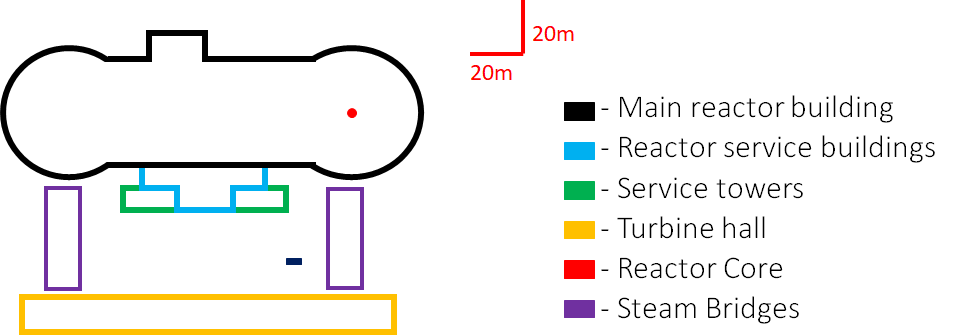
\includegraphics[width=1.0\linewidth]{wylfaReactorBuildings/wylfaTrace+key.png}
 \captionof{figure}{Trace of the Wylfa reactor site (figure \ref{fig:googleMapsDetector}) showing the key buildings that cast muon shadows onto the detector. } 
 \label{fig:wylfaTraceOfBuildings}
\end{figure}

\begin{figure}[H]
 \centering
 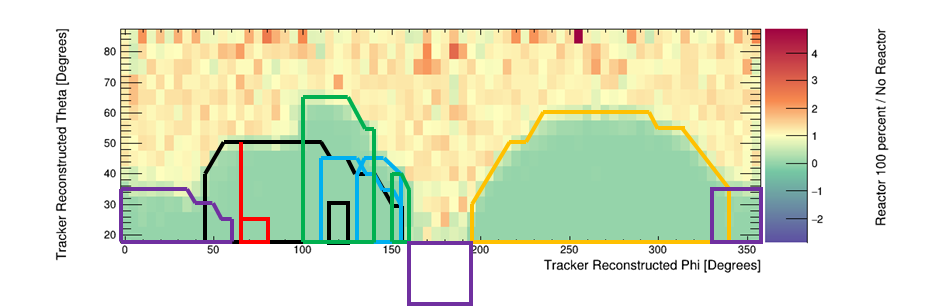
\includegraphics[width=1.0\linewidth]{panoramicReults/SimulatedBuildingsThetaPhiNew.png}
 \captionof{figure}{Ratio of simulated Geant 4 data with and without the shadow. The shadows are shown in green (ratio $<$ 1). In order to determine which components of the shadow are caused by which building each building was simulated on its own. The key to the outlines is the same as in figure \ref{fig:wylfaTraceOfBuildings}.}
 \label{fig:simulatedBuildingsThetaPhi}
\end{figure}

\begin{figure}[H]
 \centering
 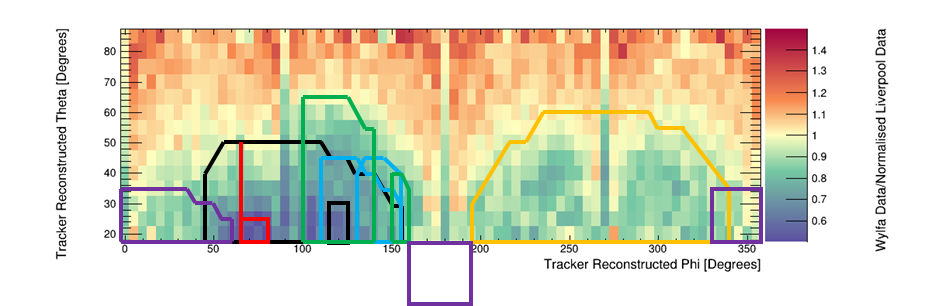
\includegraphics[width=1.0\linewidth]{panoramicReults/MeasuredBuildingsThetaPhiNew.png}
 \captionof{figure}{Ratio of the Wylfa and Liverpool data shadows are seen with a values $\sim$ $<=$ 1 coloured yellow and green. The components of the reactor shadows match very closely with figure \ref{fig:simulatedBuildingsThetaPhi}. The key to the outlines is the same as in figure \ref{fig:wylfaTraceOfBuildings}. } 
 \label{fig:measuredBuildingsThetaPhi}
\end{figure}

\begin{figure}[H]
 \centering
 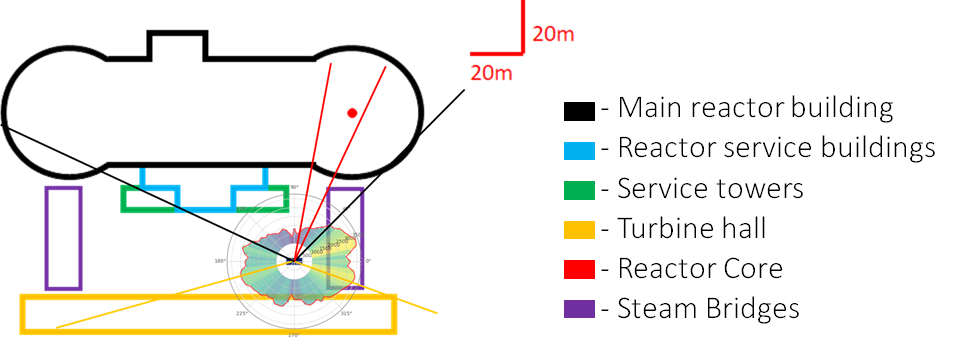
\includegraphics[width=1.0\linewidth]{wylfaReactorBuildings/wylfaTrace+overlay+key.png}
 \captionof{figure}{Figure \ref{fig:wylfaTraceOfBuildings} with an overlay of measured data from the Wylfa reactor site highlighting the main reactor building turbine hall and reactor core area.} 
 \label{fig:wylfaTraceOfBuildings+overlay}
\end{figure}

\section{Application to Reactor Monitoring} \label{sec:ApplicationToReactorMonitoring}
Anti-neutrinos cannot be blocked by any material, due to their small cross section of the order 10$^{-42}$ cm$^2$ \cite{Vogel_1999}. It is even possible for neutrinos to traverse through planet Earth without interacting with any matter \hl{citation needed}. As a result the only way to potentially mask the number of anti-neutrinos being measured by an anti-neutrino detector is to physically move the detector. For example moving the detector twice as close would correlate to an anti-neutrino rate four times higher if the power generation were to remain consistent via the squared law. However, it would be possible for an unscrupulous reactor site to reduce power by a factor 4 and in such an instance and prevent burn up of illicit materials \hl{citation needed}. But if the VIDARR detector were to switch into cosmic mode for 1 hour every week this would not be possible as the change in position would be highly noticeable and 1 week is not enough to produce illicit bomb grade material \hl{citation needed}. 

\section{Conclusion} \label{sec:Conclusion}
 The VIDARR prototype has measured the shadows at the Wylfa reactor site and these measurements correspond very well with simulated building positions. These simulated building positions have then helped to inform building heights and specific features at the Wylfa site including the shadow of the reactor core and the reactor core apparatus. In addition this is possible with only $\sim$ 1 hours worth of data at the Wylfa reactor site.

\section{Appendix} \label{sec:appendix}
\begin{figure}[H]
 \centering
 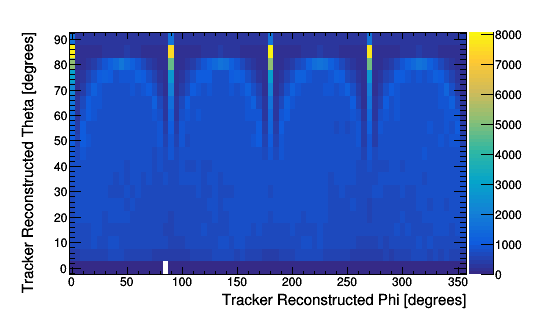
\includegraphics[width=0.7\linewidth]{ReconstructedPhiTheta/pvsTFiduicalHemisphere.png}
 \captionof{figure}{Simulated cosmic hemisphere for $\phi$ vs $\theta$ to show that the effects seen in figures \ref{fig:simulatedBuildingsThetaPhi} and \ref{fig:measuredBuildingsThetaPhi} are not a result of the cosmic tracker malfunctioning.} 
 \label{fig:pvstFiducialHem}
\end{figure}

\begin{figure}[H]
 \centering
 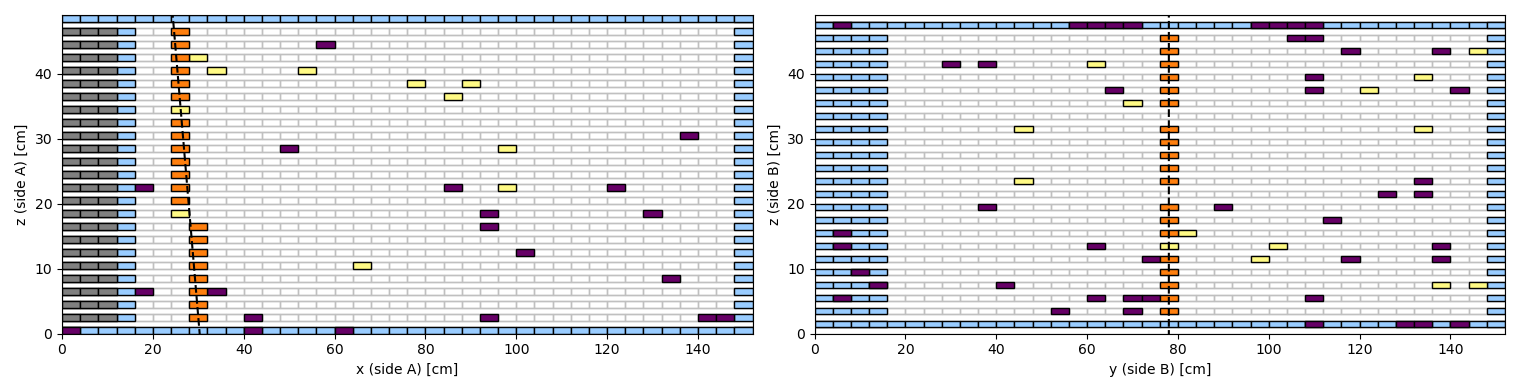
\includegraphics[width=1.0\linewidth]{testEventNewScheme.png}
 \captionof{figure}{An example event to show how the inside of the detector looks. orange is signal yellow noise, purple dead channels, grey un-instrumented, blue fiduicalised channels.}
 \label{fig:testEventNewScheme}
\end{figure}

\begin{figure}[H]
 \centering
 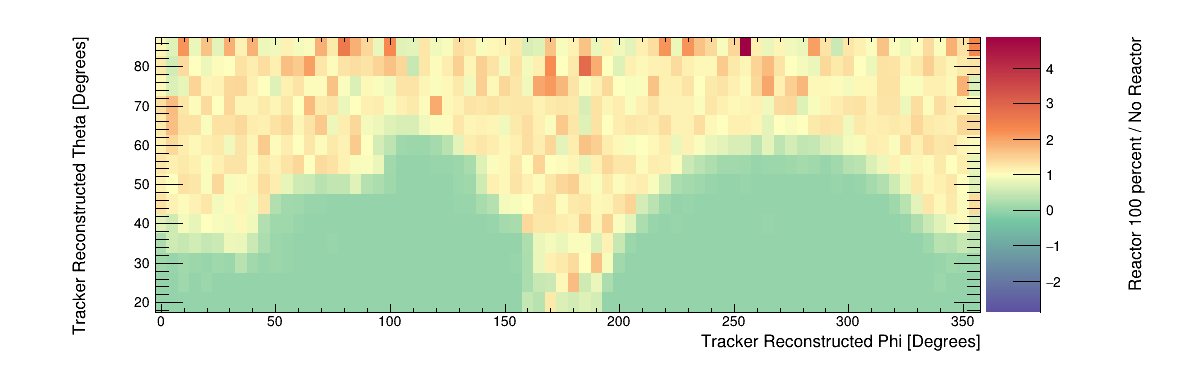
\includegraphics[width=1.0\linewidth]{panoramicReults/wylfaUpdatedGeomWithSteam100Percent.png}
 \captionof{figure}{figure \ref{fig:simulatedBuildingsThetaPhi} without the colour boxes showing the components of the shadows.} 
 \label{fig:wylfaSimulatedPvtNoBoxes}
\end{figure}

\begin{figure}[H]
 \centering
 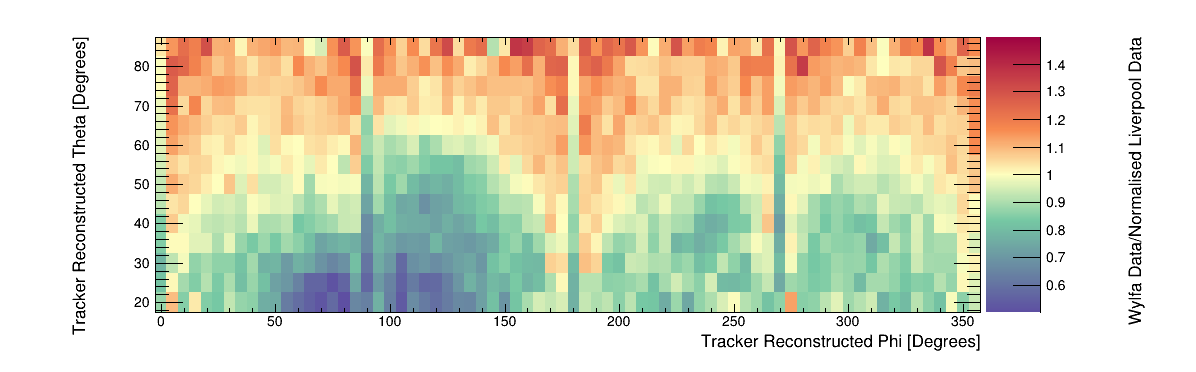
\includegraphics[width=1.0\linewidth]{panoramicReults/4CutRatioWylfaDivLivWide.png}
 \captionof{figure}{figure \ref{fig:measuredBuildingsThetaPhi} without the coloured boxes showing the components of the shadows.} 
 \label{fig:wyflaMeasuredPvtNoBoxes}
\end{figure}

\begin{figure}[H]
\centering
\begin{subfigure}{.5\textwidth}
  \centering
  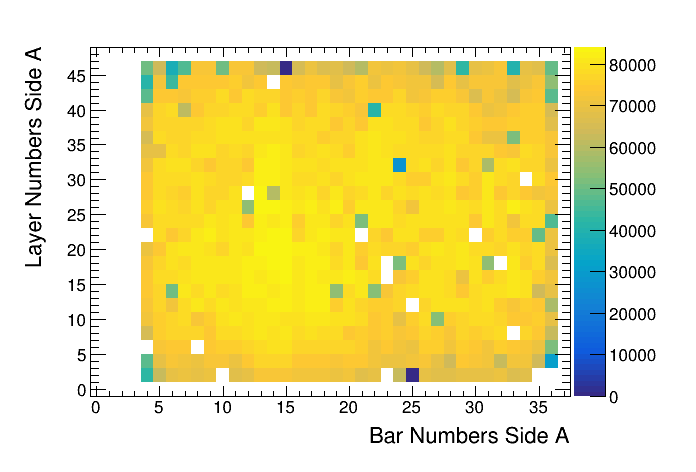
\includegraphics[width=\linewidth]{sidesAB/liverpoolSideAHits.png}
  \captionsetup{width=.9\linewidth}
  \caption{Side A bars and layers hit at the University of Liverpool.}
  \label{subFig:pvtLiverpool}
\end{subfigure}%
\begin{subfigure}{.5\textwidth}
  \centering
  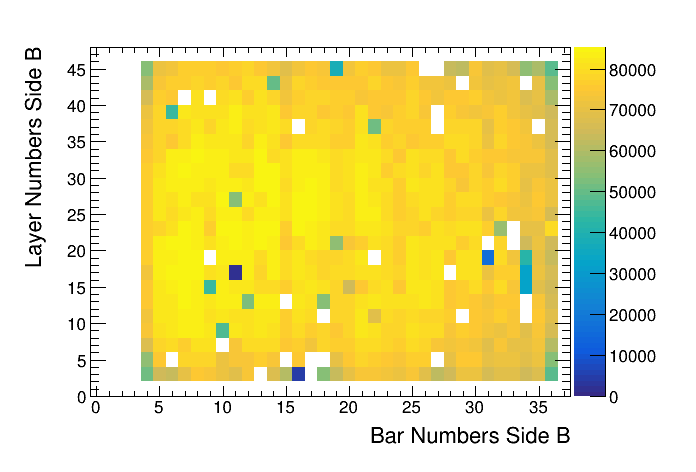
\includegraphics[width=\linewidth]{sidesAB/liverpoolSideBHits.png}
  \captionsetup{width=.9\linewidth}
  \caption{Side B bars and layers hit at the University of Liverpool.}
  \label{subFig:pvtWylfa}
\end{subfigure}
\caption{Sides A and B cosmic hits at University of Liverpool mostly uniform slightly cool at the corners.}
\label{fig:pvtWylfaAndLiverpool}
\end{figure}

\begin{figure}[H]
\centering
\begin{subfigure}{.5\textwidth}
  \centering
  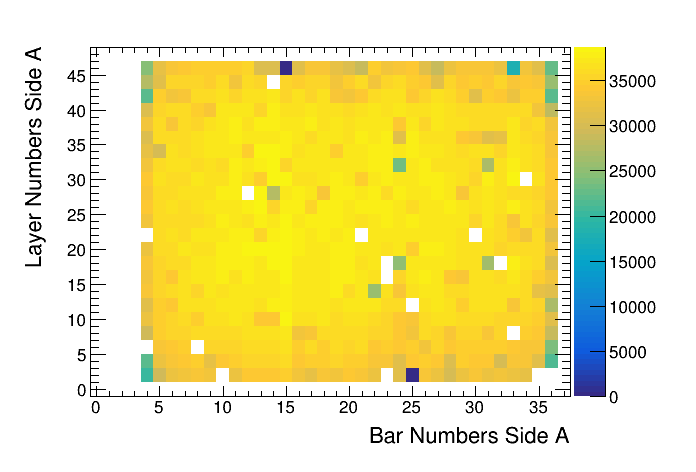
\includegraphics[width=\linewidth]{sidesAB/sideABarsAndLayersWylfa.png}
  \captionsetup{width=.9\linewidth}
  \caption{Side A bars and layers hit at the Wylfa reactor site.}
  \label{subFig:pvtLiverpool}
\end{subfigure}%
\begin{subfigure}{.5\textwidth}
  \centering
  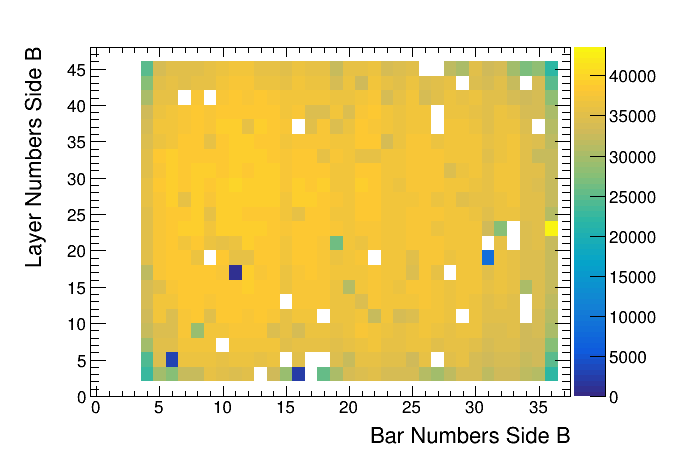
\includegraphics[width=\linewidth]{sidesAB/sideBBarsAndLayersWylfa.png}
  \captionsetup{width=.9\linewidth}
  \caption{Side B bars and layers hit at the Wylfa reactor site.}
  \label{subFig:pvtWylfa}
\end{subfigure}
\caption{Sides A and B cosmic hits at the Wylfa reactor site mostly uniform slightly cool at the corners. Side B has a noisy channel at bar no. 36 but this shouldn't affect results.}
\label{fig:pvtWylfaAndLiverpool}
\end{figure}

%\bibliography{refs} 
%\bibliographystyle{ieeetr}
\printbibliography


\end{document}
